\documentclass[10pt]{article}
\usepackage[polish]{babel}
\usepackage[utf8]{inputenc}
\usepackage[T1]{fontenc}
\usepackage{amsmath}
\usepackage{amsfonts}
\usepackage{amssymb}
\usepackage[version=4]{mhchem}
\usepackage{stmaryrd}
\usepackage{graphicx}
\usepackage[export]{adjustbox}
\graphicspath{ {./images/} }

\begin{document}
\begin{enumerate}
  \item Liczby \(a, b, c\) to dodatnie liczby wymierne spełniające równość \(a^{2}+b^{2}+c^{2}=a b c\).\\
Udowodnij, że liczba \(\sqrt{\left(a^{3}+b c\right)\left(b^{3}+c a\right)\left(c^{3}+a b\right)}\) jest wymierna.
  \item Dany jest prostokąt \(A B C D\). Punkt \(P\) jest środkiem boku \(A B\), a punkt Q jest rzutem prostokątnym punktu C na prostą PD. Udowodnij, że trójkąt QBC jest równoramienny.
  \item Na rysunku wszystkie okręgi mają promień 1, a trójkąt jest prostokątny. Jakie jest pole trójkąta?\\
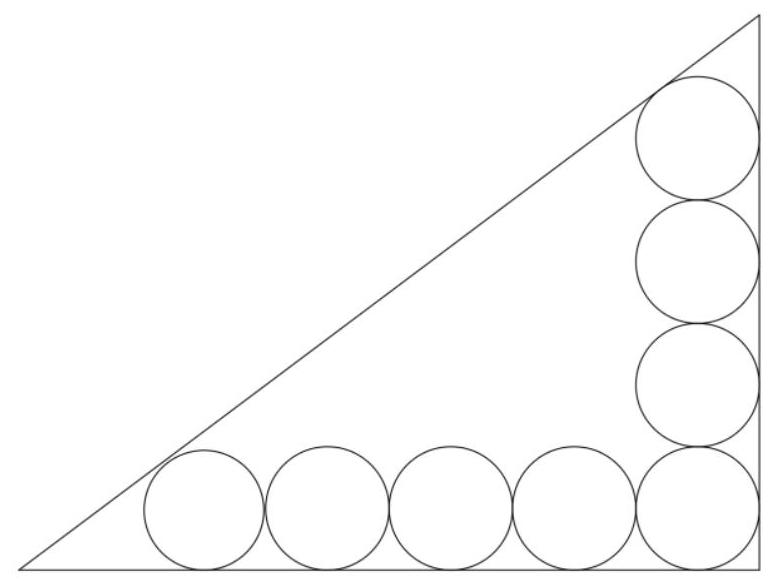
\includegraphics[max width=\textwidth, center]{2024_11_21_67112a28987ab362ffb2g-1}
\end{enumerate}

\end{document}